\section{Introduction}
\label{sec:intro}

Test-time adaptation (TTA) corrects for distribution shift by updating a model's parameters online using only unlabeled test data.
The dominant evaluation protocol measures how much closed-set accuracy improves on corrupted in-distribution images.
This metric answers one question well: \emph{does the model classify shifted images more accurately after adaptation?}
It is blind to a second question that matters equally in real deployment: \emph{does the model still know what it does not know?}

In realistic deployment, test streams are not curated.
Batches mix corrupted in-distribution (ID) samples with out-of-distribution (OOD) samples from categories the model has never seen.
A model must simultaneously (1) classify shifted ID images correctly---what TTA optimizes---and (2) detect OOD images as anomalous and abstain.
Entropy-minimizing TTA \citep{tent} pursues objective (1) by sharpening every prediction toward its current most likely class.
This conflicts directly with objective (2): sharpening OOD predictions eliminates the uncertainty that OOD detectors rely on.

\begin{figure}[t]
  \centering
  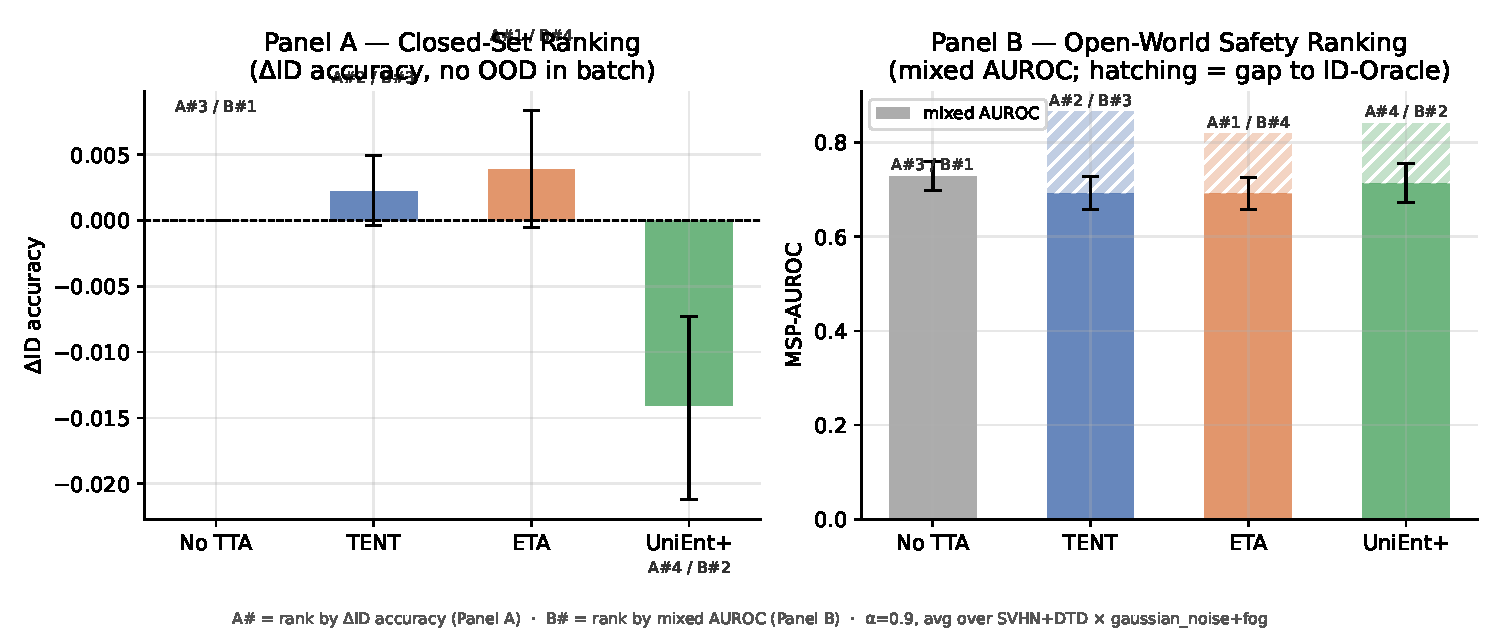
\includegraphics[width=\linewidth]{figures/fig1_ranking_reversal.pdf}
  \caption{%
    \textbf{Closed-set TTA rankings invert open-world safety rankings.}
    \emph{Left (Panel A)}: Closed-set metric---change in ID accuracy on corrupted CIFAR-10 ($\alpha{=}0.9$, gaussian noise). ETA ranks first, UniEnt+ last.
    \emph{Right (Panel B)}: Open-world metric---mixed-stream AUROC. No adaptation ranks first; ETA and TENT fall \emph{below} the no-adaptation baseline. The method that tops the closed-set leaderboard (ETA) ranks joint-last by open-world AUROC (averaged at $\alpha{=}0.9$).
    Rank numbers overlaid on each bar.
  }
  \label{fig:ranking_reversal}
\end{figure}

Prior work on open-world TTA \citep{owttt,unient,rosetta} acknowledges that OOD contamination degrades adaptation quality and proposes methods to mitigate it.
We ask a different question: \emph{how much does each method actually solve?}
We introduce a \emph{paired contamination protocol} that measures this directly, and apply it as a diagnostic across existing methods including those explicitly designed for open-world settings.

\paragraph{Contributions.}
\begin{enumerate}[leftmargin=*,topsep=2pt,itemsep=1pt]
  \item \textbf{Paired contamination protocol.} We define a contamination cost $\gap = \DeltaA(\idonly) - \DeltaA(\mixed)$ by pairing an ID-only oracle against realistic mixed-batch adaptation on identical test streams. The forfeit fraction $\forfeit = \gap / \DeltaA(\idonly)$ measures what fraction of the achievable OOD-detection benefit is lost to contamination. Across 4 OOD datasets, 2 TTA methods, 4 ID fractions $\alpha$, and 3 OOD detectors, the gap is significant in 27/32 cells ($p < 0.05$); $\forfeit > 1$ in most cells, meaning mixed TTA leaves OOD detection \emph{worse} than no adaptation.

  \item \textbf{Mechanism decomposition.} A four-condition experimental control isolates OOD gradient contamination as the dominant mechanism (+120--456\% of the total gap). BatchNorm statistics exposure to OOD inputs, decoupled from the gradient, is not harmful---it is actively beneficial. This overturns the prior hypothesis that shared batch statistics are the culprit.

  \item \textbf{Cross-method safety audit.} Applying the paired protocol across four method families---No TTA, TENT, ETA, and UniEnt+---reveals a ranking reversal: ETA ranks first by closed-set ID-accuracy gain but joint-last by mixed-stream AUROC (tied with TENT). In our heavy-contamination audit ($\alpha = 0.9$, averaged across OOD datasets and corruptions), the no-adaptation baseline attains the highest mixed-stream AUROC, exceeding all entropy-minimizing TTA methods tested. UniEnt+, designed explicitly for open-world streams, partially recovers but does not close the gap.

  \item \textbf{Reporting standard.} We recommend that TTA papers targeting open-world deployment report the paired contamination gap alongside ID accuracy, making the adaptation--abstention tradeoff visible.
\end{enumerate}

\paragraph{Scope and limitations.} The \idonly{} oracle is a diagnostic tool, not a deployable method: it requires ground-truth ID/OOD labels---precisely what an OOD detector is designed to produce. Our contribution is the gap $\gap$ as an interpretable bound, not a system one can deploy. We do not propose a new adaptation algorithm; we provide the evaluation tool that reveals how much each existing algorithm actually solves. Limitations are discussed in Section~\ref{sec:conclusion}.
